\documentclass[10pt,letterpaper]{article}
\usepackage[letterpaper,margin=0.65in,headheight=14pt,footskip=0.34in]{geometry}
\usepackage[T1]{fontenc}
\usepackage{lmodern}
\usepackage{microtype}
\usepackage{setspace}
\usepackage{booktabs,longtable,tabularx,array}
\usepackage{graphicx}
\usepackage{enumitem}
\usepackage{caption}
\usepackage{tikz}
\usetikzlibrary{arrows.meta,positioning,shapes.geometric}
\usepackage[hidelinks]{hyperref}
\usepackage{fancyhdr}
\usepackage{needspace}
\hypersetup{pdftitle={Helping Hand T2 Beta Test Plan},pdfauthor={Helping Hand Team}}
\setstretch{1.02}
\setlength{\parindent}{0pt}
\setlength{\parskip}{2pt plus 1pt minus 1pt}
\setlength{\emergencystretch}{2em}
\setlist{nosep,leftmargin=*}
\captionsetup{font=small,labelfont=bf,justification=raggedright,singlelinecheck=false}
\renewcommand{\arraystretch}{1.08}
\setlength{\tabcolsep}{4pt}
\setlength{\LTpre}{3pt}
\setlength{\LTpost}{4pt}
\pagestyle{fancy}
\fancyhf{}
\fancyhead[L]{Helping Hand | T2 Beta Test Plan}
\fancyhead[R]{CEN4908C}
\fancyfoot[C]{\thepage}
\renewcommand{\headrulewidth}{0.35pt}
\newcolumntype{Y}{>{\raggedright\arraybackslash}X}
\newcolumntype{P}[1]{>{\raggedright\arraybackslash}p{#1}}

\begin{document}
\hypersetup{pageanchor=false}
\begin{titlepage}
\thispagestyle{empty}
\vspace*{0.55in}
{\large University of Florida\par}
{\normalsize Herbert Wertheim College of Engineering\par}
\vspace{0.88in}
{\Huge\bfseries T2: Beta Test Plan\par}
\vspace{0.16in}
{\LARGE Helping Hand\par}
\vspace{0.34in}
\rule{\textwidth}{0.6pt}
\vspace{0.20in}
\begin{tabularx}{\textwidth}{@{}P{1.5in}Y@{}}
\textbf{Project} & Helping Hand \\
\textbf{Assignment} & T2: Beta Test Plan \\
\textbf{Team members} & Gael Garcia; Kali Schuchhardt; Brian Paz; Srinitha Srikanth \\
\textbf{Course} & Senior Design 2, CEN4908C, Section 23346 \\
\textbf{Instructor} & Jeremiah Blanchard \\
\textbf{Date} & October 2, 2026 \\
\end{tabularx}
\vspace{0.20in}
\rule{\textwidth}{0.6pt}
\vfill
\begin{minipage}{\textwidth}
\small This plan defines observable system behavior and reproducible checks for the Helping Hand wearable-assisted ASL learning system. Historical alpha evidence is separated from beta procedures that remain unrun; proposed acceptance targets are labeled as such.
\end{minipage}
\end{titlepage}
\hypersetup{pageanchor=true}

\section{Alpha Test Results}
\subsection{Confirmed results and evidence limits}
The table reports repository and team-note evidence available for this plan. A procedure in the alpha plan is not proof that the procedure ran. No current beta hardware or route result is inferred from an older build.

\begin{longtable}{@{}P{1.15in}P{3.28in}P{2.55in}@{}}
\caption{Documented alpha evidence and its effect on beta testing}\label{tab:alpha}\\
\toprule
\textbf{Evidence / date} & \textbf{Confirmed outcome} & \textbf{Beta consequence}\\\midrule
\endfirsthead
\toprule\textbf{Evidence / date} & \textbf{Confirmed outcome} & \textbf{Beta consequence}\\\midrule
\endhead
\bottomrule\endlastfoot
Automated checks, Sep. 10, 2026; \texttt{cce9d38} & Flutter analysis and 16 Flutter tests passed; Android debug APK, Feather ESP32-S3 PlatformIO build, and 23 backend tests passed. TFLite produced three non-failing deprecation warnings. Firmware report: 37.6\% RAM and 83.9\% configured application flash. & Re-run build and test suites against the beta source; the alpha checks do not validate the new routes, assembled glove, or live Firebase behavior. \\
Firebase alpha setup & README records project setup, Anonymous Authentication, Firestore availability, owner-only rules deployed/read back, and emulator display of Synced. & Test current email/password accounts, UID isolation, offline recovery, and cold restart using a controlled test environment. \\
Historical physical demonstration & Archived demonstrations show flex changes received on Android over BLE with static prediction and confidence displayed. & Repeat with the present glove assembly; measure packet delivery, disconnect recovery, and route updates under sustained use. \\
Record Signs pilot, Sep. 17, 2026 & One signer produced 35 static-sign trials and 5,518 valid BLE frames at neutral orientation, with five flex and six IMU channels; observed rate was about 39.7--40.5 Hz. & Treat this as a static pilot only. It is not a word dataset or model-accuracy evidence; beta recording checks must validate export integrity and metadata. \\
Account work, Oct. 1 notes & Team notes report email/password account creation and sign-in. Eight repository UID-isolation tests passed at \texttt{873b589} with local stores and fake remotes. & Keep live Firestore cross-account, rules, offline, and restart checks separate; these outcomes were not covered by the repository tests. \\
UI and practice routes & Visual redesign commit \texttt{9c5caab} passed analysis, production web build, and five temporary responsive/interaction checks. Route commit \texttt{d581d19} passed targeted Flutter analysis. & Exercise all routes on target devices. Temporary widget checks and static analysis are not device usability or BLE integration results. \\
\end{longtable}\subsection{Lessons carried into beta}
The documented record shows a useful static baseline and a small, single-signer recording pilot, but not a multi-signer dynamic-word evaluation. The current glove assembly has not been regression-tested; the firmware has a documented startup wait tied to serial readiness; sustained phone-side BLE loss, exact IMU identity, and magnetometer capability remain unconfirmed. Email/password sign-in and repository-level UID separation have evidence, while live Firestore isolation and recovery do not.

The beta implementation adds account flows, UID-scoped local progress, separate letter/number/word practice routes, and route-level refreshes from the shell-owned BLE connection. The record does not attribute these changes to specific measured participant feedback, so this plan makes no such claim. Beta testing consequently emphasizes standalone boot, sensor and BLE measurement, navigation and Back behavior, Retry and completion transitions, live account isolation/sync, export integrity, independent usability, and a gated dynamic-word pipeline. Word pages are accessible UI; word recognition and word completion remain unintegrated.

\section{Expected Behavior}
\subsection{System overview and state transitions}
The Feather ESP32-S3 reads five flex channels and a six-axis accelerometer/gyroscope, runs the existing static 36-class TFLite baseline, and sends timestamped/sequenced data over BLE. The Flutter app owns the connection and tracker, displays current link/prediction state, and presents a dedicated route for each selected target. Progress is stored locally for the authenticated Firebase UID and synchronized asynchronously to Firestore. Record Signs data is exported for the team dataset workflow; raw sensor sequences do not belong in learner progress. The eight displayed words are provisional candidates; there is no dynamic inference or word-completion write in the current app.

\begin{figure}[ht]
\centering
\resizebox{0.96\textwidth}{!}{%
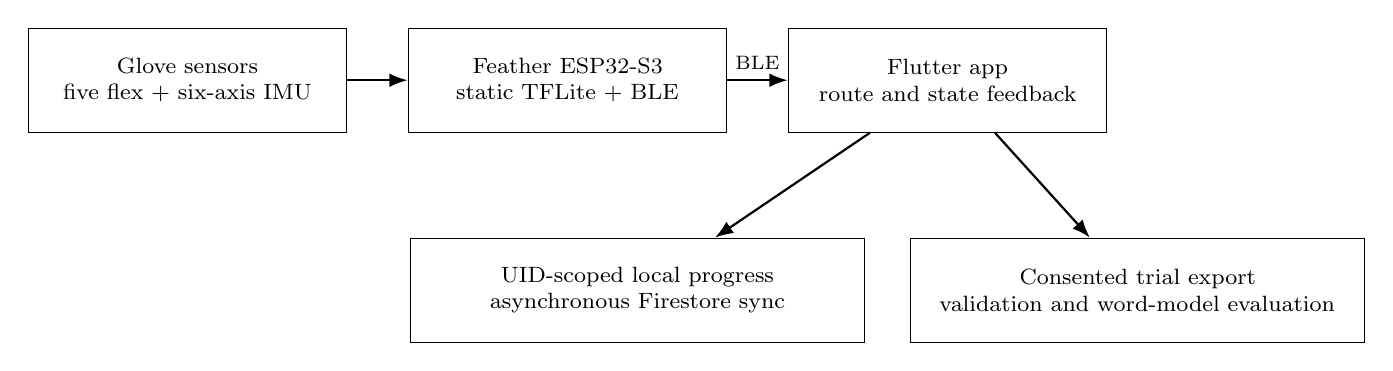
\begin{tikzpicture}[x=1in,y=1in,
 b/.style={draw,align=center,text width=1.5in,minimum height=0.52in,font=\footnotesize},
 c/.style={draw,align=center,text width=2.18in,minimum height=0.52in,font=\footnotesize},
 a/.style={-{Latex},thick}]
\node[b] (sensor) at (0,0) {Glove sensors\\five flex + six-axis IMU};
\node[b] (board) at (1.9,0) {Feather ESP32-S3\\static TFLite + BLE};
\node[b] (app) at (3.8,0) {Flutter app\\route and state feedback};
\node[c] (progress) at (2.25,-1.05) {UID-scoped local progress\\asynchronous Firestore sync};
\node[c] (dataset) at (4.75,-1.05) {Consented trial export\\validation and word-model evaluation};
\draw[a] (sensor)--(board);
\draw[a] (board)--node[above,font=\scriptsize]{BLE}(app);
\draw[a] (app)--(progress);
\draw[a] (app)--(dataset);
\end{tikzpicture}}
\caption{System paths and beta boundary. The word-model branch is planned data work, not a validated runtime feature.}
\label{fig:system}
\end{figure}

\begin{longtable}{@{}P{0.78in}P{3.27in}P{2.88in}@{}}
\caption{Observable expected behavior and verification link}\label{tab:behavior}\\
\toprule\textbf{ID} & \textbf{Expected behavior} & \textbf{Observable output / test}\\\midrule
\endfirsthead\toprule\textbf{ID} & \textbf{Expected behavior} & \textbf{Observable output / test}\\\midrule\endhead\bottomrule\endlastfoot
HW-01 & With the identified power source and no serial host, the board boots, initializes sensors, and advertises the glove. Voltage/current are within the documented ratings of the actual source and board. & Boot time, current/voltage, reset count, source identity; HW-01. \\
HW-02 & Each flex channel responds to its mapped finger; IMU values are finite and respond to motion. Absolute yaw is claimed only if the installed sensor supports it. & Raw channel values, timestamps, sensor identity and mapping; HW-02. \\
BLE-01/02 & The app scans, connects, subscribes, parses complete packets, and stops presenting stale data as live. Timeout, permission, Bluetooth-off, disconnect, and retry states provide recoverable feedback. & Scan/connect/first-packet times, IDs, packet age, parse errors and reconnects; BLE-01/02. \\
NAV-01/03 & Home and bottom navigation reach the intended destinations. Every target opens its own practice route; toolbar and Android Back return to the same picker and scroll position without duplicate pages. & Route/target title, origin, restored position, stack/crash count; NAV-01--03. \\
LIVE-01/03 & The visible route refreshes from the one shell-owned BLE connection. Retry clears an in-progress hold. A letter/number completes once only for a matching label at confidence $\geq80\%$, at least five packets and $\geq750$ ms, with no gap $>250$ ms. Back ends the active practice session; hidden routes cannot award progress. & Prediction, confidence, packet sequence/timing, hold/reset state, progress delta; LIVE-01--03. \\
AUTH-01/03 & Firebase Authentication owns credentials. Sign-in, invalid credentials, reset and account linking produce recoverable, non-revealing feedback. Progress remains scoped to the authenticated UID. & Auth result, UID alias, session restoration, sanitized error; AUTH-01--03. \\
PROG-01/05 & A qualifying static practice updates only the signed-in user's local progress and `users/{uid}/progress/current`. Local progress remains usable offline, restores after relaunch, and syncs without duplicate/lost completion. Tapping a target alone awards nothing. & Before/after local and remote snapshots, UID path, timestamps and sync status; PROG-01--05. \\
REC-01 & Recording is blocked until required metadata and fresh complete sensor input exist. Save and discard remain distinct. Export preserves raw trial content and metadata for the team pipeline without placing raw sequences in account progress. & Readiness reason, trial count, export hashes/schema and validator result; REC-01. \\
WORD-01 & A word route shows the selected target and connection state but no fabricated match, confidence, hold, or word completion from the static classifier. & Target, route, connection, exception log and before/after progress; WORD-01. \\
ML-01/02 & Word recognition is not presented as available until reviewed vocabulary, consented multi-signer data, leakage-safe evaluation, runtime validation, and acceptance gates are met. & Vocabulary/data manifest, split hashes, held-signer metrics, model/runtime identity; ML-01/02. \\
UI-01 & Controls remain reachable and readable at supported viewport sizes and large text; screen-reader labels identify the target and navigation actions. & Overflow/clipping checklist, touch size and task outcomes; UI-01. \\
\end{longtable}\subsection{Decision rules}
For static practice, tile selection selects a target but does not complete it. A prediction is eligible only when its label equals the active A--Z/0--9 target, confidence is at least 80\%, five or more consecutive valid packets span at least 750 ms, and no inter-packet gap exceeds 250 ms. Any failed condition resets the hold; one qualifying hold records exactly one completion. Retry clears only the current hold, not previously saved progress. Leaving the practice route ends eligibility until the learner re-enters.

For words, the same static output is never treated as a word result. The current valid outcome is target display plus connection feedback. Recognition and word progress require a reviewed vocabulary, a trained sequence model, a defined runtime and passing ML-02 gates. For cloud progress, local state remains authoritative for immediate UI feedback; remote failure is visible and retryable, not silently treated as synced.

\section{Test Procedures}
\subsection{Execution rules and reference configuration}
Use an Android beta build of package \texttt{1.0.0+1} and the Feather ESP32-S3 as the reference application/board configuration. The T1 reference phone is Fairphone Gen 6 / Android 15; record the actual phone and OS for each run. The current implementation reference is route commit \texttt{d581d19}. Before a run, identify the installed IMU, firmware revision, power source and rating, app artifact/hash, Firebase environment, date, tester and independent reviewer. A configuration difference is allowed if recorded; unknown firmware or sensor identity is recorded as unknown and cannot support a sensor-specific claim.

Use the Firebase emulator or designated test accounts in project \texttt{helping-hand-83137}; do not alter production rules or use real participant data without consent. Use pseudonymous signer IDs. Capture raw data only for consented recording tests and retain the original export. At each run's start, clear or snapshot the test account's progress, reset the app to the stated route, synchronize phone/packet timestamps, and verify logger storage. At the end, preserve logs, restore the app/account state, and record defects before retesting.

The procedures below have not been executed as a complete beta campaign. Record each as Pass, Fail, Blocked, or Not run; Blocked is not a pass. A test passes only if every listed criterion is met. Do not change a threshold after viewing results without revising/versioning this plan and documenting why. T1 values below are proposed acceptance targets, not beta measurements.

\subsection{Hardware and BLE}
\textbf{HW-01 -- Power and standalone boot} \hfill{\footnotesize\textit{Not run}}\par\vspace{0pt}
\fontsize{8.6pt}{9.7pt}\selectfont\renewcommand{\arraystretch}{0.98}\begin{longtable}{@{}P{1.34in}P{5.72in}@{}}\toprule

\textbf{Test field} & \textbf{Procedure record}\\\midrule
\endfirsthead
\toprule
\textbf{Test field} & \textbf{Procedure record}\\\midrule
\endhead
\midrule\multicolumn{2}{r}{Continued on next page}\\
\endfoot
\bottomrule\endlastfoot
Purpose / behavior requirement & Check safe power behavior and independence from a serial host.\\
Equipment / setup / preconditions & \textbf{Equipment:} Fully assembled glove, identified battery or supply, meter/logger, Android phone with BLE scan capture; board and source ratings available. \newline \textbf{Preconditions:} Inspect wiring and insulation; identify source voltage/capacity and board input limits. If ratings or source identity cannot be established, record Blocked for electrical acceptance. \\
Procedure & 1) With the board idle, measure voltage/current. 2) Perform five cold power cycles with USB serial disconnected. 3) For each cycle, measure time to BLE advertisement. 4) Measure current during a stable ten-minute stream. Record temperature observations and any resets.\\
Expected result & Board starts and advertises without a serial monitor, remains stable while streaming, and shows no damage or abnormal heating.\\
Metric / pass-fail & Pass if 5/5 advertisements occur within 15 s (T1), there are zero resets, and all measured values remain within identified component/source ratings. If battery capacity is known, estimate runtime as rated capacity divided by measured average current and report the method; do not substitute an assumed capacity.\\
Data / logs & Source/board labels and ratings, idle/start/stream V and I, five boot times, resets, temperature observations, firmware revision, photos and logger file.\\
\bottomrule\end{longtable}\normalsize\vspace{1pt}

\textbf{HW-02 -- Sensor mapping and static baseline} \hfill{\footnotesize\textit{Not run}}\par\vspace{0pt}
\fontsize{8.6pt}{9.7pt}\selectfont\renewcommand{\arraystretch}{0.98}\begin{longtable}{@{}P{1.34in}P{5.72in}@{}}\toprule

\textbf{Test field} & \textbf{Procedure record}\\\midrule
\endfirsthead
\toprule
\textbf{Test field} & \textbf{Procedure record}\\\midrule
\endhead
\midrule\multicolumn{2}{r}{Continued on next page}\\
\endfoot
\bottomrule\endlastfoot
Purpose / behavior requirement & Verify flex/IMU input response and protect the existing 36-class static regression baseline.\\
Equipment / setup / preconditions & \textbf{Equipment:} Glove, raw packet logger, reference phone/app, one practiced signer, frozen A--Z/0--9 label order, and known sensor markings. \newline \textbf{Preconditions:} HW-01 passes. Record rest baseline and verify the logger's timestamps and units before collecting trials. \\
Procedure & 1) At rest, capture 10 s of each channel. 2) Bend each finger separately five times, then together; record raw values. 3) Rotate each accessible IMU axis in both directions five times. 4) Collect five trials for each of the 36 static labels. 5) Evaluate a frozen representative subset and the complete set; preserve a confusion matrix.\\
Expected result & Each flex channel responds primarily to its mapped finger; all emitted IMU values are finite and change with motion. All 36 labels have reported trial counts and predictions; no class is omitted silently.\\
Metric / pass-fail & Flex excursion is at least 100 ADC counts and five times that channel's rest peak-to-peak noise; T1 IMU targets are rest mean 0.8--1.2 g and rotation peak at least 20 deg/s on an accessible axis. Static T1 gates: representative-subset top-1 at least 80\%; full characterization reports overall top-1 and macro F1 against initial targets of 70\% and 0.65. Any unverified channel mapping or missing label fails the corresponding check.\\
Data / logs & Sensor part/marking, channel map, raw samples/timestamps, rest noise, per-trial label/prediction/confidence, counts, top-1, macro F1 and confusion matrix.\\
\bottomrule\end{longtable}\normalsize\vspace{1pt}

\textbf{BLE-01 -- Discovery, permission and connection timeout} \hfill{\footnotesize\textit{Not run}}\par\vspace{0pt}
\fontsize{8.6pt}{9.7pt}\selectfont\renewcommand{\arraystretch}{0.98}\begin{longtable}{@{}P{1.34in}P{5.72in}@{}}\toprule

\textbf{Test field} & \textbf{Procedure record}\\\midrule
\endfirsthead
\toprule
\textbf{Test field} & \textbf{Procedure record}\\\midrule
\endhead
\midrule\multicolumn{2}{r}{Continued on next page}\\
\endfoot
\bottomrule\endlastfoot
Purpose / behavior requirement & Verify discovery, subscription, timeout feedback and recovery when permission or Bluetooth is unavailable.\\
Equipment / setup / preconditions & \textbf{Equipment:} Reference Android phone, powered glove, screen recording, synchronized clock and app event log. \newline \textbf{Preconditions:} HW-01 passes; begin on the BLE Testing screen with app permissions documented. \\
Procedure & 1) Perform ten scan/select/connect attempts and time advertisement, connection, subscription and first valid packet. 2) Deny the required permission and retry. 3) Disable Bluetooth and retry. 4) Restore permission/Bluetooth and reconnect after each negative case.\\
Expected result & App explains each recoverable condition, does not crash or remain indefinitely loading, and resumes only after permission/radio restoration and a valid packet.\\
Metric / pass-fail & Pass if discovery succeeds within 15 s in at least 9/10 attempts and connection/subscription within 10 s in at least 9/10 (T1). Each negative case must expose an error/action state and recover without app restart; record any configured timeout and fail if it never resolves.\\
Data / logs & Attempt-level timestamps, permission/radio state, link state, first packet, user-visible message, app/OS version and screen video.\\
\bottomrule\end{longtable}\normalsize\vspace{1pt}

\textbf{BLE-02 -- Packet quality, sustained stream and reconnect} \hfill{\footnotesize\textit{Not run}}\par\vspace{0pt}
\fontsize{8.6pt}{9.7pt}\selectfont\renewcommand{\arraystretch}{0.98}\begin{longtable}{@{}P{1.34in}P{5.72in}@{}}\toprule

\textbf{Test field} & \textbf{Procedure record}\\\midrule
\endfirsthead
\toprule
\textbf{Test field} & \textbf{Procedure record}\\\midrule
\endhead
\midrule\multicolumn{2}{r}{Continued on next page}\\
\endfoot
\bottomrule\endlastfoot
Purpose / behavior requirement & Measure end-to-end device-to-phone delivery, parsing, timing and asynchronous recovery.\\
Equipment / setup / preconditions & \textbf{Equipment:} Glove, phone/app, raw packet logger with sequence/timestamp capture, stable power source. \newline \textbf{Preconditions:} BLE-01 passes; confirm expected channel count and logger clock before starting. \\
Procedure & 1) Stream for ten minutes while moving fingers and navigating between BLE Testing, picker and practice routes. 2) Inject or observe three controlled disconnects. 3) Restore the link and verify fresh data on each reconnect. 4) Compare sequence IDs and received frames with the expected 40 Hz schedule.\\
Expected result & Complete packets update the visible app; malformed, duplicate or decreasing IDs are not accepted as fresh live data. Disconnect state is visible and new data resumes after reconnection.\\
Metric / pass-fail & T1 gates: at least 95\% of 24,000 expected frames received, effective average at least 38 Hz, at least 99\% of received notifications parse completely, missing IDs no more than 5\%, no duplicate/decreasing ID accepted, and 3/3 reconnects within 15 s. Zero crash, firmware reset or unexplained disconnect in the ten-minute run.\\
Data / logs & Original packet capture, expected/received counts, rates, gaps, parse errors, sequence anomalies, disconnect/reconnect times, route changes and build ID.\\
\bottomrule\end{longtable}\normalsize\vspace{1pt}

\subsection{Navigation, live feedback and word boundary}
\textbf{NAV-01 to NAV-03 -- Entry points, target routes and Back} \hfill{\footnotesize\textit{Not run}}\par\vspace{0pt}
\fontsize{8.6pt}{9.7pt}\selectfont\renewcommand{\arraystretch}{0.98}\begin{longtable}{@{}P{1.34in}P{5.72in}@{}}\toprule

\textbf{Test field} & \textbf{Procedure record}\\\midrule
\endfirsthead
\toprule
\textbf{Test field} & \textbf{Procedure record}\\\midrule
\endhead
\midrule\multicolumn{2}{r}{Continued on next page}\\
\endfoot
\bottomrule\endlastfoot
Purpose / behavior requirement & Verify learner navigation, all target routes, route state restoration and system Back.\\
Equipment / setup / preconditions & \textbf{Equipment:} Current Android beta build, phone screen recording, route checklist, one test account; glove optional except where live completion is observed. \newline \textbf{Preconditions:} Sign in to a clean test account. Reset to Home and record the selected bottom-navigation tab and scroll positions. \\
Procedure & NAV-01: open Alphabet, Numbers and Words from each Home learning-path row, then open every bottom-navigation destination. NAV-02: tap all 26 letters, 10 numbers and eight displayed words; verify each route title/target, then use toolbar Back. NAV-03: scroll Alphabet to its last row and Words to Drink; repeat open/Back using both toolbar Back and Android system Back for 20 cycles.\\
Expected result & Each destination/target opens the correct screen; practice is a separate route, not embedded in the picker. Back returns to its originating picker/tab and preserves scroll position. Words remains accessible without a false recognition result.\\
Metric / pass-fail & NAV-01: all six documented entry points reach the correct destination. NAV-02: 44/44 choices show the matching title and return to the origin. NAV-03: 20/20 repeated cycles restore the correct route/scroll position, with zero duplicate pages or crashes. A hidden practice route cannot award progress after Back.\\
Data / logs & Route checklist, target IDs/titles, Back method, origin/return tab, scroll positions, cycle count, completion deltas, crashes and screen recording.\\
\bottomrule\end{longtable}\normalsize\vspace{1pt}

\textbf{LIVE-01 to LIVE-03 -- Route updates, Retry and static completion} \hfill{\footnotesize\textit{Not run}}\par\vspace{0pt}
\fontsize{8.6pt}{9.7pt}\selectfont\renewcommand{\arraystretch}{0.98}\begin{longtable}{@{}P{1.34in}P{5.72in}@{}}\toprule

\textbf{Test field} & \textbf{Procedure record}\\\midrule
\endfirsthead
\toprule
\textbf{Test field} & \textbf{Procedure record}\\\midrule
\endhead
\midrule\multicolumn{2}{r}{Continued on next page}\\
\endfoot
\bottomrule\endlastfoot
Purpose / behavior requirement & Verify that the pushed practice page reflects the shell-owned BLE connection and applies the static completion gate exactly once.\\
Equipment / setup / preconditions & \textbf{Equipment:} Phone/app, glove or controlled packet source, logger, test account with progress snapshot. \newline \textbf{Preconditions:} BLE-02 passes; select Letter A, record its pre-test completion state, and keep exactly one BLE connection active. \\
Procedure & LIVE-01: produce A, another label, then disconnect/reconnect while the route stays open. LIVE-02: cause an incomplete hold, tap Retry, then repeat after a completed hold. LIVE-03: submit wrong label, confidence below 80\%, four matching packets, hold shorter than 750 ms, and a gap above 250 ms; finally submit a valid stable A and repeat its packets. Use a fresh pre-test snapshot for each independent invalid case.\\
Expected result & The visible route refreshes prediction/confidence/connection state without a second BLE connection. Retry clears current hold/match feedback but not saved completion. Invalid inputs never complete; one qualifying hold completes once. Back ends eligibility so later packets cannot complete a hidden target.\\
Metric / pass-fail & Route feedback reflects each controlled state change within 1 s (T1 responsiveness target). Valid completion requires matching label, confidence $\geq80\%$, at least five consecutive packets spanning $\geq750$ ms, and no gap $>250$ ms. Pass iff every invalid case adds zero and the valid case adds exactly one; repeat packets add zero additional completions.\\
Data / logs & Packet trace, target/label/confidence, timestamps/gaps, connection count, Retry time, hold state, screen video and before/after local/remote progress.\\
\bottomrule\end{longtable}\normalsize\vspace{1pt}

\textbf{WORD-01 -- Word-page UI without false recognition} \hfill{\footnotesize\textit{Not run}}\par\vspace{0pt}
\fontsize{8.6pt}{9.7pt}\selectfont\renewcommand{\arraystretch}{0.98}\begin{longtable}{@{}P{1.34in}P{5.72in}@{}}\toprule

\textbf{Test field} & \textbf{Procedure record}\\\midrule
\endfirsthead
\toprule
\textbf{Test field} & \textbf{Procedure record}\\\midrule
\endhead
\midrule\multicolumn{2}{r}{Continued on next page}\\
\endfoot
\bottomrule\endlastfoot
Purpose / behavior requirement & Confirm accessible word pages do not route static character output into word recognition or award unsupported word progress.\\
Equipment / setup / preconditions & \textbf{Equipment:} Phone/app, test account, screen recording and optional static glove stream. \newline \textbf{Preconditions:} Save a progress snapshot; record the candidate list as provisional: hello, thank\_you, please, sorry, yes, no, eat and drink. \\
Procedure & Open all eight word rows, verify each target title, use Retry where available, and stream static letter/number predictions. Compare local and Firestore progress before/after.\\
Expected result & Correct target and connection state may display. No word match/confidence/hold is claimed from the static classifier; no word completion is stored; no invalid-target exception occurs.\\
Metric / pass-fail & Pass only if all eight routes render the selected target and zero word completions or false matches occur. Any display or progress delta attributable to a static prediction fails.\\
Data / logs & Vocabulary/list version, route checklist, before/after progress snapshot, exception log, build/model identifiers and video.\\
\bottomrule\end{longtable}\normalsize\vspace{1pt}

\subsection{Authentication, progress and data integrity}
\textbf{AUTH-01 to AUTH-03 -- Account lifecycle and credential errors} \hfill{\footnotesize\textit{Not run}}\par\vspace{0pt}
\fontsize{8.6pt}{9.7pt}\selectfont\renewcommand{\arraystretch}{0.98}\begin{longtable}{@{}P{1.34in}P{5.72in}@{}}\toprule

\textbf{Test field} & \textbf{Procedure record}\\\midrule
\endfirsthead
\toprule
\textbf{Test field} & \textbf{Procedure record}\\\midrule
\endhead
\midrule\multicolumn{2}{r}{Continued on next page}\\
\endfoot
\bottomrule\endlastfoot
Purpose / behavior requirement & Check email/password account creation, session restoration, invalid credentials/reset, and linking of an existing anonymous alpha session.\\
Equipment / setup / preconditions & \textbf{Equipment:} Firebase emulator or designated test project, two team-controlled accounts, app log with secrets redacted. \newline \textbf{Preconditions:} Confirm test environment and account cleanup path; never record passwords or reset tokens. \\
Procedure & AUTH-01: create account A, sign out, force-stop/relaunch and sign in again. AUTH-02: submit an invalid password and request password reset for a controlled address; inspect user-visible feedback. AUTH-03: start from a test anonymous session with progress, link email credentials, then sign out/in and inspect UID and progress.\\
Expected result & A is created once and signs in after restart. Invalid credentials are rejected with recoverable, non-enumerating feedback; reset flow responds without revealing account existence. Linking preserves the same UID and associated test progress where supported.\\
Metric / pass-fail & Pass iff all three flows complete with correct auth state, no crash, no plaintext secret in Firestore/logs, and AUTH-03 retains the expected UID/progress. Record reset-email delivery as environment-dependent; do not pass if the flow gives no observable result.\\
Data / logs & Pseudonymous account aliases, auth-state transitions, UID before/after linking, sanitized errors, reset request/result, environment and app artifact.\\
\bottomrule\end{longtable}\normalsize\vspace{1pt}

\textbf{PROG-01 to PROG-05 -- Persistence, sync and UID isolation} \hfill{\footnotesize\textit{Not run}}\par\vspace{0pt}
\fontsize{8.6pt}{9.7pt}\selectfont\renewcommand{\arraystretch}{0.98}\begin{longtable}{@{}P{1.34in}P{5.72in}@{}}\toprule

\textbf{Test field} & \textbf{Procedure record}\\\midrule
\endfirsthead
\toprule
\textbf{Test field} & \textbf{Procedure record}\\\midrule
\endhead
\midrule\multicolumn{2}{r}{Continued on next page}\\
\endfoot
\bottomrule\endlastfoot
Purpose / behavior requirement & Verify that progress matches the learner-visible state, remains usable offline, synchronizes to the correct UID and is protected by Firestore rules.\\
Equipment / setup / preconditions & \textbf{Equipment:} Emulator or authorized Firebase test project, two accounts A/B, phone, network toggle, Firestore emulator/rules test path, local and remote snapshot tools. \newline \textbf{Preconditions:} AUTH-01 passes. Record empty baseline progress for A and B and verify account UID aliases. \\
Procedure & PROG-01: complete one eligible letter online and compare UI with `users/{uid}/progress/current`; tap an uncompleted tile separately. PROG-02: sign out A, sign in B on the same phone, and compare both states. PROG-03: go offline, complete one item, restart offline, reconnect and retry sync. PROG-04: test owner, other-UID and unauthenticated get/create/update/delete using emulator rules. PROG-05: force-stop after online completion, relaunch, then repeat after offline completion/reconnect.\\
Expected result & Only the eligible accepted practice changes progress. B cannot read or modify A. Offline local progress remains navigable and later syncs without loss or duplicate. Rules reject cross-user and unauthenticated operations; correct owner access succeeds.\\
Metric / pass-fail & Local state restores within 3 s and stable-network Synced state appears within 15 s (T1). Pass iff UI/local/remote values agree after sync; tile taps change nothing; no cross-UID leakage, duplicate/lost completion, or unauthorized rules operation. If no controlled Firebase environment is available, mark PROG-04 Blocked.\\
Data / logs & Account aliases/UIDs, environment and rules revision, before/after UI/local/remote snapshots, network/restart/sync times, request outcomes and sanitized errors.\\
\bottomrule\end{longtable}\normalsize\vspace{1pt}

\textbf{REC-01 -- Record, discard, export and validate} \hfill{\footnotesize\textit{Not run}}\par\vspace{0pt}
\fontsize{8.6pt}{9.7pt}\selectfont\renewcommand{\arraystretch}{0.98}\begin{longtable}{@{}P{1.34in}P{5.72in}@{}}\toprule

\textbf{Test field} & \textbf{Procedure record}\\\midrule
\endfirsthead
\toprule
\textbf{Test field} & \textbf{Procedure record}\\\midrule
\endhead
\midrule\multicolumn{2}{r}{Continued on next page}\\
\endfoot
\bottomrule\endlastfoot
Purpose / behavior requirement & Verify recording readiness, invalid-input handling, save/discard distinction, export integrity and backend validation.\\
Equipment / setup / preconditions & \textbf{Equipment:} Glove/phone, consented pseudonymous signer if human data is captured, approved metadata schema, storage, export transfer route and backend validator. \newline \textbf{Preconditions:} BLE-02 passes; tester has authority to record and knows the approved metadata fields. Use synthetic data for malformed-input tests. \\
Procedure & Attempt start with each required metadata field missing and with stale/incomplete packets. Record one valid trial and save it; record a second and discard with a reason. Export CSV/JSON to the phone, transfer through the approved team path, compare hashes, then run the valid export and a deliberately malformed fixture through the validator.\\
Expected result & Invalid starts remain blocked with a reason. Saved trial appears once; discarded trial is absent from training exports and its reason is retained. Export is readable and unchanged in transfer; malformed data is categorized, not silently accepted. Raw sequences are absent from account progress.\\
Metric / pass-fail & Pass iff every missing/stale case is rejected, saved count increases by one, discarded count by zero, transfer hashes match, valid export has zero schema errors and malformed fixture is flagged. Any unconsented human recording fails the run.\\
Data / logs & Consent reference (not identity), metadata manifest, packet freshness, save/discard counts/reason, filenames/schema, hashes, transfer record, validator report and build ID.\\
\bottomrule\end{longtable}\normalsize\vspace{1pt}

\subsection{Dynamic word and usability evaluation}
\textbf{ML-01 -- Reviewed word dataset} \hfill{\footnotesize\textit{Not run}}\par\vspace{0pt}
\fontsize{8.6pt}{9.7pt}\selectfont\renewcommand{\arraystretch}{0.98}\begin{longtable}{@{}P{1.34in}P{5.72in}@{}}\toprule

\textbf{Test field} & \textbf{Procedure record}\\\midrule
\endfirsthead
\toprule
\textbf{Test field} & \textbf{Procedure record}\\\midrule
\endhead
\midrule\multicolumn{2}{r}{Continued on next page}\\
\endfoot
\bottomrule\endlastfoot
Purpose / behavior requirement & Build a traceable, balanced, consented sequence dataset suitable for evaluating dynamic word recognition.\\
Equipment / setup / preconditions & \textbf{Equipment:} Glove/logger, secure team storage, written collection script, consent materials, ASL-qualified reviewer and data manifest. \newline \textbf{Preconditions:} Reviewer approves glosses, signing instructions and immutable vocabulary version before collection. Current eight candidates are not an approved vocabulary. \\
Procedure & Collect pilot trials across five signers, eight candidate words and four orientations (neutral, pitch-up, roll-left, yaw-right), five trials per cell. Inspect packet completeness and protocol; then collect at least 20 accepted trials per cell for a full target. Preserve rejected trials with reasons and never overwrite raw captures.\\
Expected result & Every accepted sequence has signer pseudonym, word/version, orientation, trial ID, timestamps, sensor channels, consent reference and validator status. The dataset is balanced to the selected target or gaps are explicitly listed.\\
Metric / pass-fail & T1 collection targets: 800 pilot trials at five signers; full target 3,200 at five signers or 2,560 at four. Pass only after reviewer approval, consented coverage, complete metadata, and validated per-cell counts. If reviewer/consent/vocabulary is unavailable, mark Blocked.\\
Data / logs & Vocabulary/reviewer version, consent log, pseudonyms, raw and manifest hashes, per-cell accepted/rejected counts, exclusions/reasons, firmware and sensor IDs.\\
\bottomrule\end{longtable}\normalsize\vspace{1pt}

\textbf{ML-02 -- Leakage-safe model and runtime gate} \hfill{\footnotesize\textit{Blocked}}\par\vspace{0pt}
\fontsize{8.6pt}{9.7pt}\selectfont\renewcommand{\arraystretch}{0.98}\begin{longtable}{@{}P{1.34in}P{5.72in}@{}}\toprule

\textbf{Test field} & \textbf{Procedure record}\\\midrule
\endfirsthead
\toprule
\textbf{Test field} & \textbf{Procedure record}\\\midrule
\endhead
\midrule\multicolumn{2}{r}{Continued on next page}\\
\endfoot
\bottomrule\endlastfoot
Purpose / behavior requirement & Evaluate dynamic recognition on unseen signers and determine whether any model is suitable for the declared runtime.\\
Equipment / setup / preconditions & \textbf{Equipment:} ML-01 validated dataset, fixed preprocessing/training environment, candidate TCN, CNN-GRU and CNN-LSTM implementations, selected phone or ESP32 runtime. \newline \textbf{Preconditions:} ML-01 passes; freeze dataset and code hashes, vocabulary, split, random seeds and metric script before training. The current app has no integrated dynamic word model, so this test is presently Blocked. \\
Procedure & Split complete trials by signer before fitting preprocessing. Fit scaling/window settings on train data only. Compare candidates with same split/seeds; report user-dependent and held-signer results, per-orientation confusion, top-1/top-5, macro F1, model size and latency. Convert the best qualifying candidate to TFLite and run end-to-end inference on the selected runtime while retaining static regression checks.\\
Expected result & No signer or trial leaks across held-out evaluation. Results are reproducible from hashes/seeds. If no candidate clears every gate, retain static baseline and report dynamic recognition as unavailable.\\
Metric / pass-fail & T1 proposed gates: held-signer top-1 $\geq70\%$, macro F1 $\geq0.65$, top-5 $\geq90\%$ for more than five classes, worst-orientation drop $\leq15$ percentage points; median inference $<100$ ms and P95 $<150$ ms; displayed suggestion P95 $\leq300$ ms after a complete window. Zero leakage and successful end-to-end runtime are required.\\
Data / logs & Dataset/split/code hashes, seeds, environment, vocabulary, confusion matrices, all metrics, orientation counts, model hash/size, runtime, latency traces and static-baseline regression.\\
\bottomrule\end{longtable}\normalsize\vspace{1pt}

\textbf{UI-01 -- Responsive and independent usability} \hfill{\footnotesize\textit{Not run}}\par\vspace{0pt}
\fontsize{8.6pt}{9.7pt}\selectfont\renewcommand{\arraystretch}{0.98}\begin{longtable}{@{}P{1.34in}P{5.72in}@{}}\toprule

\textbf{Test field} & \textbf{Procedure record}\\\midrule
\endfirsthead
\toprule
\textbf{Test field} & \textbf{Procedure record}\\\midrule
\endhead
\midrule\multicolumn{2}{r}{Continued on next page}\\
\endfoot
\bottomrule\endlastfoot
Purpose / behavior requirement & Check whether learners can use primary routes and controls independently and whether layout/accessibility survives supported display settings.\\
Equipment / setup / preconditions & \textbf{Equipment:} Current Android beta build, 320 px and 375 px phone viewports, landscape/tablet if supported, largest system text setting, TalkBack, reduced motion and moderator. Three non-team participants with consent for observation. \newline \textbf{Preconditions:} Test account is reset; participants receive only task prompts, not step-by-step instructions. Do not collect unnecessary identifying information. \\
Procedure & Ask each participant to sign in, find an assigned letter/number/word, enter and leave practice with Back, connect/retry, and locate progress/sync state without coaching. Inspect Home, pickers, short and long target pages at each viewport/text setting; verify control size and TalkBack labels.\\
Expected result & All controls remain visible/reachable, selected targets are understandable, Back/Retry labels are announced, no clipped content/overflow blocks a task, and no coaching is needed for critical navigation.\\
Metric / pass-fail & T1 proposed usability gate: at least 80\% of tasks complete without coaching; each critical task succeeds for at least 2/3 participants; median ease rating at least 4/5. No clipped controls at largest text; interactive targets at least 48 logical dp. Report each participant/task separately.\\
Data / logs & Pseudonymous participant codes, task success/time/errors, ease ratings, viewport/text/accessibility settings, control measurements, moderator notes and defect IDs.\\
\bottomrule\end{longtable}\normalsize\vspace{1pt}

\subsection{Run record and exit decision}
For every run, record test ID and attempt, date/time, tester and reviewer, app artifact/hash, phone/OS, board model, IMU identity, firmware version, power source, Firebase environment, measured values, Pass/Fail/Blocked/Not run, defect and retest link, and evidence filenames. Never log passwords, reset tokens, or direct participant identifiers. Keep failed captures and rerun under a new attempt number.

The beta is ready for release-candidate consideration only after hardware/stream, all 44 navigation choices, live-route feedback, static completion gates, account/rules/progress, recording/export, word-page false-positive protection and independent usability have recorded results. Dynamic recognition is a separate release gate: ML-01 and ML-02 must pass before the app claims word recognition or word completion. Any unmet metric is reported as measured; a blocked or unrun procedure is not described as a pass.

\small\textit{Evidence sources:} repository README and M3 alpha record; beta build-status and test-working-notes documents; T1 Alpha Test Plan (proposed gates); recorded-data and preprocessing documentation; Issue 7 IMU word-level research.

\end{document}
